%%%%%%%%%%%%%%%%%%%%%%%%%%%%%%%%%%%%%%%%%
% Beamer Presentation
% LaTeX Template
% Version 1.0 (10/11/12)
%
% This template has been downloaded from:
% http://www.LaTeXTemplates.com
%
% License:
% CC BY-NC-SA 3.0 (http://creativecommons.org/licenses/by-nc-sa/3.0/)
%
%%%%%%%%%%%%%%%%%%%%%%%%%%%%%%%%%%%%%%%%%

%----------------------------------------------------------------------------------------
%	PACKAGES AND THEMES
%----------------------------------------------------------------------------------------

\documentclass{beamer}

\mode<presentation> {

% The Beamer class comes with a number of default slide themes
% which change the colors and layouts of slides. Below this is a list
% of all the themes, uncomment each in turn to see what they look like.

%\usetheme{default}
%\usetheme{AnnArbor}
%\usetheme{Antibes}
%\usetheme{Bergen}
%\usetheme{Berkeley}
%\usetheme{Berlin}
%\usetheme{Boadilla}
%\usetheme{CambridgeUS}
%\usetheme{Copenhagen}
%\usetheme{Darmstadt}
%\usetheme{Dresden}
%\usetheme{Frankfurt}
%\usetheme{Goettingen}
%\usetheme{Hannover}
%\usetheme{Ilmenau}
%\usetheme{JuanLesPins}
%\usetheme{Luebeck}
\usetheme{Madrid}
%\usetheme{Malmoe}
%\usetheme{Marburg}
%\usetheme{Montpellier}
%\usetheme{PaloAlto}
%\usetheme{Pittsburgh}
%\usetheme{Rochester}
%\usetheme{Singapore}
%\usetheme{Szeged}
%\usetheme{Warsaw}

% As well as themes, the Beamer class has a number of color themes
% for any slide theme. Uncomment each of these in turn to see how it
% changes the colors of your current slide theme.

%\usecolortheme{albatross}
%\usecolortheme{beaver}
%\usecolortheme{beetle}
%\usecolortheme{crane}
%\usecolortheme{dolphin}
%\usecolortheme{dove}
%\usecolortheme{fly}
%\usecolortheme{lily}
%\usecolortheme{orchid}
%\usecolortheme{rose}
%\usecolortheme{seagull}
%\usecolortheme{seahorse}
%\usecolortheme{whale}
%\usecolortheme{wolverine}

%\setbeamertemplate{footline} % To remove the footer line in all slides uncomment this line
%\setbeamertemplate{footline}[page number] % To replace the footer line in all slides with a simple slide count uncomment this line

%\setbeamertemplate{navigation symbols}{} % To remove the navigation symbols from the bottom of all slides uncomment this line
}

\usepackage{graphicx} % Allows including images
\usepackage{booktabs}
\usepackage{xmpmulti}
\usepackage{animate}
\usepackage{epstopdf}

\epstopdfsetup{outdir=./figures}  %Required to change filepath for .eps graphics because exectuing typesetting uses the {epstopdf} package to convert .eps graphics to .pdf format.
\graphicspath{{figures/}}	%Ensures that .eps graphics used for figures is found at the appropriate path.

 % Allows the use of \toprule, \midrule and \bottomrule in tables

%----------------------------------------------------------------------------------------
%	TITLE PAGE
%----------------------------------------------------------------------------------------

\title[Honours Project Presentation]{Linear Dispersive Waves in Optical Fibers} % The short title appears at the bottom of every slide, the full title is only on the title page

\author{Tommy Zieba} % Your name
\institute[Carleton University] % Your institution as it will appear on the bottom of every slide, may be shorthand to save space
{
Carleton University \\ % Your institution for the title page
\medskip % Your email address
}
\date{April 26, 2018} % Date, can be changed to a custom date

\begin{document}

\begin{frame}
\titlepage % Print the title page as the first slide
\end{frame}
%------------------------------------------------
\begin{frame}[fragile]
\frametitle{\textbf{Physical Properties of an Optical Fiber}}
\begin{minipage}[1.0\textheight]{\textwidth}
\begin{columns}[T]
\begin{column}{0.55\textwidth}
\begin{itemize}
\item Silica glass core surrounded by cladding.
\item Glass naturally charge neutral at rest and assumed to remain neutrally charged as light passes through it.
\item Core is isotropic, homogeneous and non-birefringent.\\
\item Core-cladding boundary at radius $a$.
\end{itemize}
\end{column}
\begin{column}{0.45\textwidth}
\vspace{-5mm}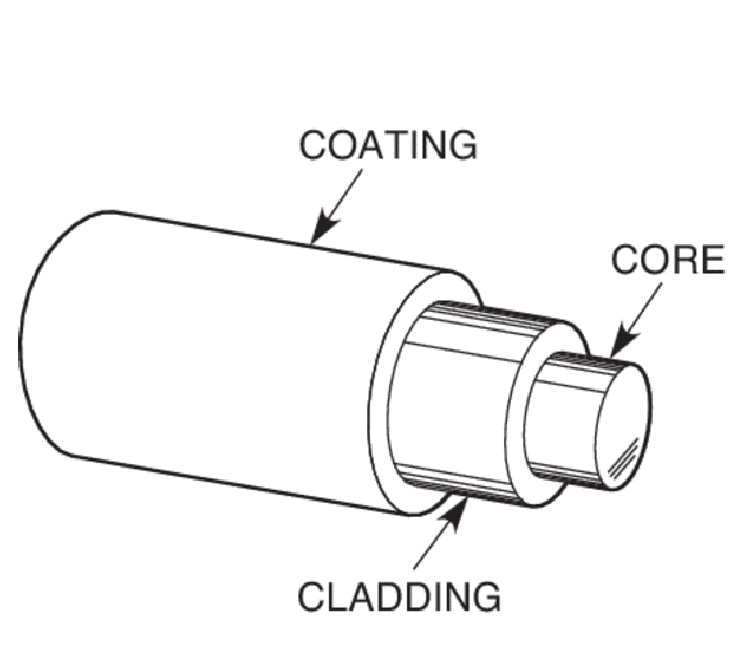
\includegraphics[width=5cm]{fiberDiagram.eps}
\tiny{\begin{verbatim}
https://www.newport.com/t/fiber-optic-basics
\end{verbatim}}
\end{column}
\end{columns}
\end{minipage}

\begin{itemize}
\item Refractive index of the core and cladding are $n_1$ and $n_0$, respectively.
\item Cladding of arbitrary radius.
\end{itemize}
\end{frame}

%2
\begin{frame}
\frametitle{\textbf{Properties of Light:} Snell's Law}
\textbf{Boundary conditions necessary for light confinement in the core are required. We investigate the properties of light at the core-cladding boundary.}
\begin{itemize}
\item Snell's Law is derived from Descarte's Law.
\item \textbf{Descarte's Law:} Sufficiently small variations in the path of light implies light travels in a straight line.
\end{itemize}
\begin{minipage}[1.0\textheight]{\textwidth}
\begin{columns}[T]
\begin{column}{0.45\textwidth}
\vspace{5mm}\begin{itemize}
\item Reflection occurs only if $$n_1>n_0,$$ $$\frac{\pi}{2}-\theta_i>\theta_c=\sin^{-1}{\left(\frac{n_0}{n_1}\right)}.$$
\end{itemize}
\end{column}
\begin{column}{0.5\textwidth}
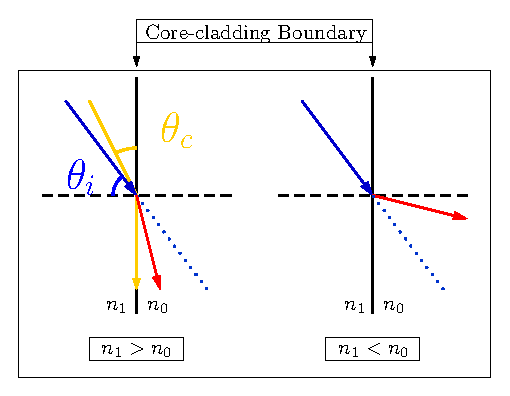
\includegraphics[width=5cm]{snellsLaw.eps}
\end{column}
\end{columns}
\end{minipage}
\end{frame}

%3
\begin{frame}
\frametitle{\textbf{Properties of Light:} Snell's Law and Goos-Hanchen Shift}
\textbf{Conclusion from Snell's law: }Cylindrical symmetry and trigonometric identities give the maximum acceptance angle,
$$\theta_{max}\leq \sin^{-1}{\sqrt{n_1^2+n_0^2}}.$$
\begin{itemize}
\item \textbf{Goos-Hanchen shift} is a lateral shift of reflected rays.
\item Electromagnetic waves have complex phase.
\item Reflected ray no longer has same complex phase.
\item Phase difference implies a lateral shift occurs.
\end{itemize}
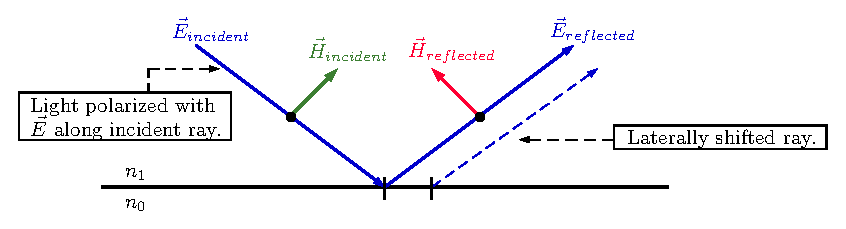
\includegraphics[width=12cm, height=3cm]{lightRayPropagation.eps}
\end{frame}

%4
\begin{frame}
\frametitle{\textbf{Electromagnetic Theory}}
\begin{itemize}
\item \textbf{Maxwell's equations:}
\begin{columns}
\column{0.5\textwidth}
\begin{gather}
\vec{\nabla}\circ\vec{D}=\rho\\
{\nabla}\circ\vec{B}=0
\end{gather}
\column{0.5\textwidth}
\begin{gather}
\vec{\nabla}\times\vec{E}=-\mu_0\frac{\partial\vec{H}}{\partial t}\\
\vec{\nabla}\times\vec{H}=\vec{J}+\frac{\partial\vec{D}}{\partial t}
\end{gather}
\end{columns}
\item Combine to obtain \textbf{Maxwell's wave equations};
$$\nabla^2\vec{E}=\mu_0 n^2(r)\varepsilon_0\frac{\partial^2\vec{E}}{\partial t^2}\qquad\mbox{and}\qquad\nabla^2\vec{H}=\mu_0 n^2(r)\varepsilon_0\frac{\partial^2\vec{H}}{\partial t^2}.$$
\item Solutions are monochromatic phasors w.r.t. time;
\begin{equation}
\vec{E}(\vec{r},t)=\vec{E}(r,\theta,z)e^{i\omega t}\qquad\mbox{and}\qquad\vec{H}(\vec{r},t)=\vec{H}(r,\theta,z)e^{i\omega t}.
\end{equation}
\end{itemize}
\end{frame}

%5
\begin{frame}
\frametitle{\textbf{Hyperbolic PDEs:} The Cauchy Problem}
\begin{itemize}
\item \textbf{Cauchy Problem:} $n^{th}$ order partial differential equation (PDE) with $m$ independent variables and specified boundary conditions (BCs).
\item Conditions specified on solution and derivatives of order $<(n-1)$. 
\item \textbf{Maxwell's wave equations:} $2^{nd}$ order linear PDEs; independent variables $(r,\theta,z,t)$.
\item \textbf{Boundary conditions:} $$E_{T}^{(core)}=E_{T}^{(cladding)}\quad\mbox{and}\quad H_{T}^{(core)}=H_{T}^{(cladding)},$$ $\forall T\in\{r,\theta,z,t\}$ satisfying $r=a$.
\end{itemize}
\end{frame}

%6
\begin{frame}
\frametitle{\textbf{Hyperbolic PDEs:} Method of Characteristics}
\begin{block}{Definition: Hyperbolic PDE}
A PDE is hyperbolic for sets of points where the Cauchy problem has a unique solution in the neighbourhood of the points on any non-characteristic hyper-plane passing though them. Unique solutions are hyper-surfaces such that the hyper-planes have at least one less independent variable.
\end{block}
\begin{itemize}
\item Method of characteristics used to find unique solution along light rays.
\item Known parametrization of solution used to determine unique solutions \textbf{or} hyperbolic regions for solutions are determined by unique parametrized hyper-planes satisfying solution uniquely.
\end{itemize}
\end{frame}

%7
\begin{frame}
\frametitle{\textbf{Applying the Method of Characteristics:} Example}
\begin{itemize}
\item \textbf{1-dimensional wave equation:}
\begin{columns}
\column{0.45\textwidth}
$$u_{tt}(x,t)-c^2u_{xx}(x,t)=0,$$ $$x\in[0,L]\subset\mathbb{R}$$ $$t\in[0,\infty)\subset\mathbb{R}$$
\column{0.45\textwidth}
\begin{gather}
u(x,0)=f(x)\nonumber\\
u_t(x,0)=g(x)\nonumber\\
u(0,t)=0\nonumber\\
u(L,t)=0\nonumber
\end{gather}
\end{columns}
\item Equivalent to $2^{nd}$ order PDE; $$\mathcal{L}[u]=a(x,t)u_{xx}+b(x,t)u_{tt}+d(x,t)u_{xt}=0,$$ with $a=1$, $b=c^2$ and $d=0$.
\item Apply parametrization $$(x,t)\mapsto(\xi,\eta);\quad\xi(x,t)=x+ct,\quad \eta(x,t)=x-ct.$$
\item Solutions necessarily hyperbolic since $b^2-4ac=c^4>0$.
\end{itemize}
\end{frame}

%8
\begin{frame}
\frametitle{\textbf{Applying the Method of Characteristics:} Example}

\begin{itemize}
\item Solution obtain by inputting parametrization into PDE is called d'Alembert's solution;
$$u(x,t)=p(x+ct)-q(x-ct)=\frac{1}{2}\Big(f\left(\xi\right)+f\left(\eta\right)\Big)+\frac{1}{2c}\int_{\eta}^{\xi}g(s)ds.$$
\end{itemize}
\begin{columns}
\column{0.5\textwidth}
\hspace{0.5cm}
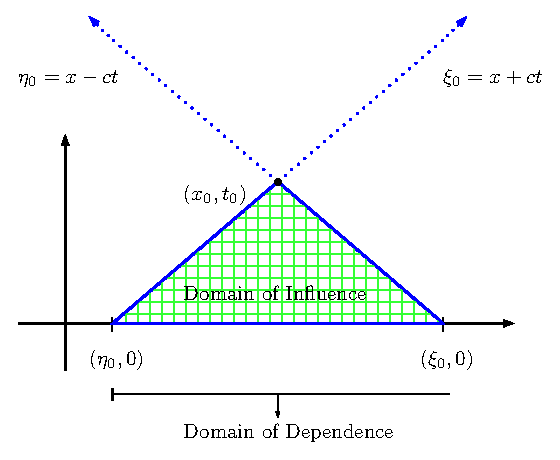
\includegraphics[width=4cm]{IBVP1.eps}
\column{0.7\textwidth}
\hspace{-1.5cm}
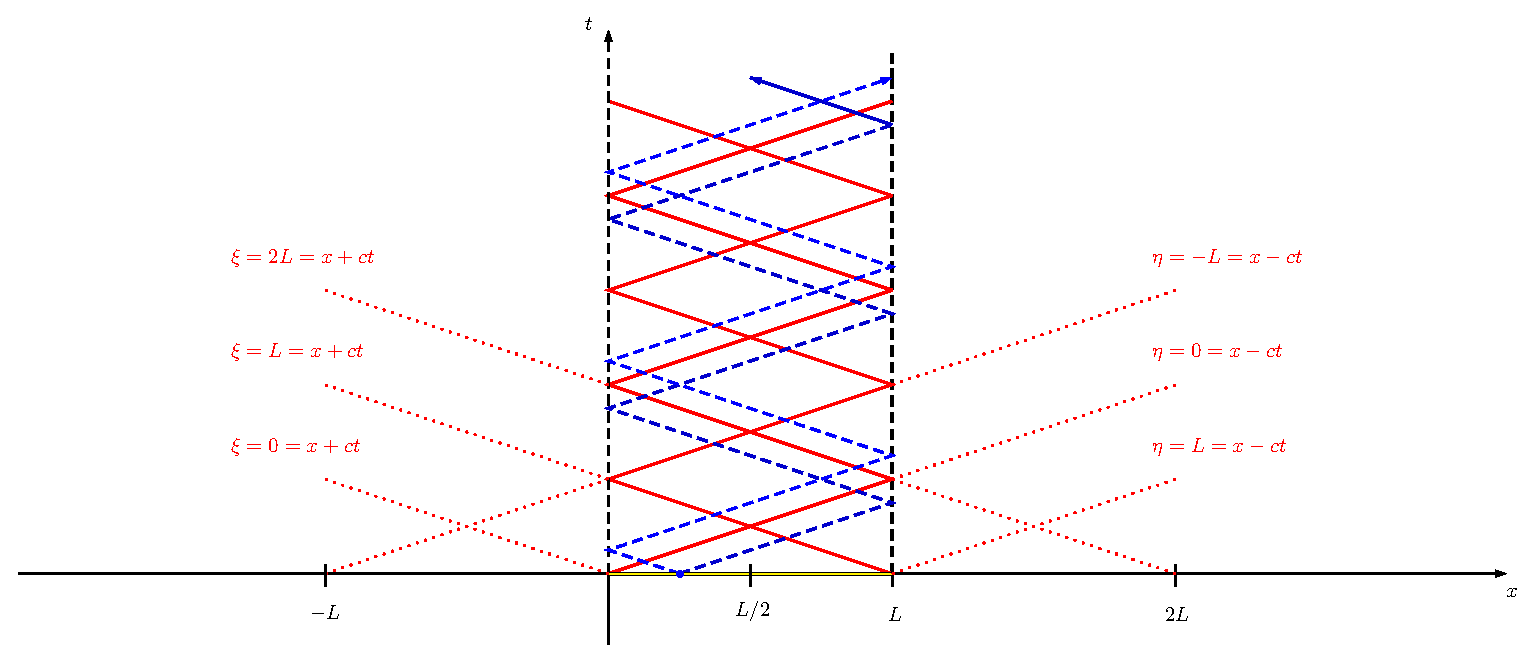
\includegraphics[width=8cm, height=4cm]{IBVP2.eps}
\end{columns}
\end{frame}

%9
\begin{frame}
\frametitle{\textbf{Dispersion:} Definition}
\begin{itemize}
\item Consider a homogeneous PDE with $4$ independent variables $(x_r,x_\theta,x_z,t)$.
\item \textbf{Dispersion} defined by solutions $u(\vec{x},t)=Ae^{i\vec{\kappa}\circ\vec{x}-i\omega t}$, $\vec{\kappa}$, $\omega$ constants.
\item Input into PDE to obtain dispersion relation $G(\omega,\kappa_r,\kappa_\theta,\kappa_z)=0$.
\item Solutions, $\omega$, are called dispersion modes.
\item Real solutions are $Re(u)=|A|\cos{(\vec{\kappa}\circ\vec{x}-\omega t+ArgA)}$.
\end{itemize}
\end{frame}

%10
\begin{frame}[fragile]
\frametitle{\textbf{Dispersion:} Phase Velocity}
\begin{itemize}
\item For each dispersion mode $\omega$, consider phase surfaces $\vartheta=\vec{\kappa}\circ\vec{x}-\omega t$.
\item \textbf{Phase velocity} is determined by the \textbf{\textit{average}} number of wavelengths per period in the direction normal to phase surfaces with respect to space.\item For fixed phase surface $\vartheta=\mbox{constant}$, this direction is $\vec{\kappa}$.
\item Average wavelength is $\lambda=2\pi\slash\ |\vec{\kappa}|$ and the average period is $2\pi\slash\omega$.
\item  Phase velocity is given by$$c(\vec{\kappa})=\frac{W(\vec{\kappa})}{|\vec{\kappa}|}\hat{\kappa}=\frac{\omega}{|\vec{\kappa}|}\hat{\kappa}.$$
\end{itemize}
\hspace{3.6cm}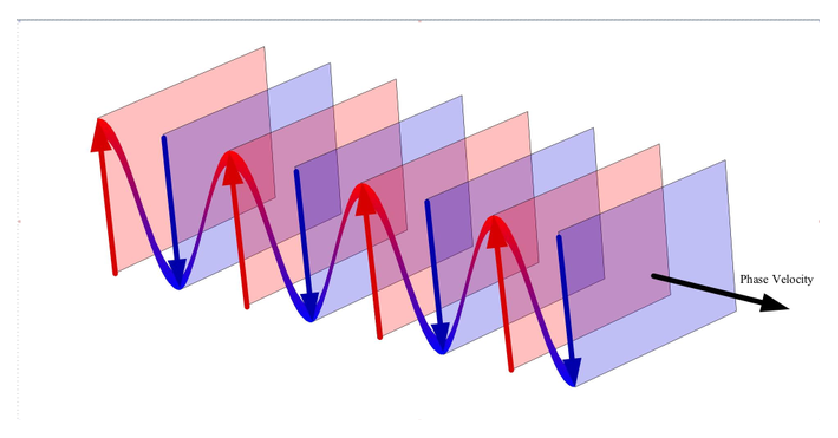
\includegraphics[width=0.4\textwidth]{planeWave.eps}
\tiny{\begin{verbatim}
                     https://courses.lumenlearning.com/boundless-physics/chapter/waves/
\end{verbatim}}
\end{frame}

%11
\begin{frame}[fragile]
\frametitle{Dispersion: Group Velocity}
\begin{itemize}
\item \textbf{Group velocity} is defined by considering \textbf{\textit{local}} wavenumber and frequency given by $$\kappa_i=\frac{\partial u}{\partial x_i}\quad\mbox{and}\quad\omega=-\frac{\partial u}{\partial t,},\quad\mbox{respectively.}$$
\item Solving for $\kappa_i(x_i,t)$ defines the group velocity component-wise as $$C_i(\vec{\kappa})=\frac{\partial W(\vec{\kappa},\vec{x},t)}{\partial\kappa_i}.$$
\end{itemize}
\hspace{2.2cm}
\includegraphics[width=75mm, height=30mm]{groupVelocity2D.eps}
\tiny{\begin{verbatim}                         http://www.phikwadraat.nl/images/article/duck/beatadd.png\end{verbatim}}
\end{frame}

%11
\begin{frame}
\frametitle{\textbf{Deriving a Solution:} Plane Wave Solution}
\vspace{1.5mm}\hspace{1.2cm}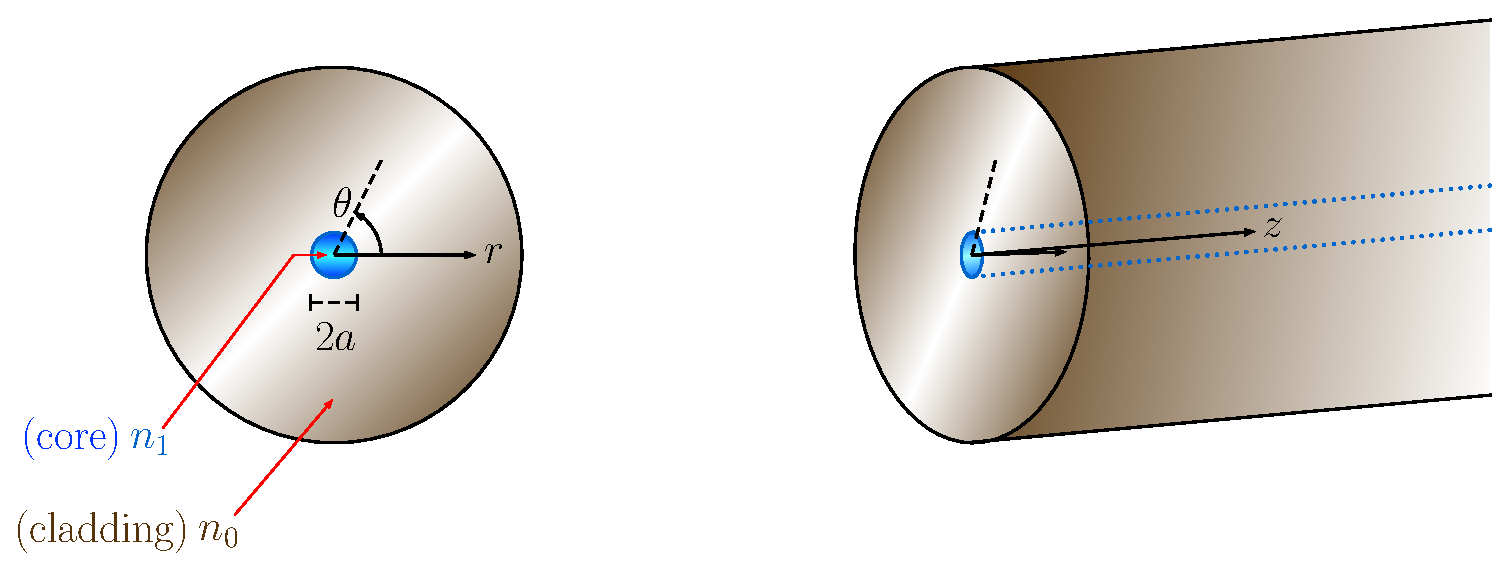
\includegraphics[width=0.75\textwidth]{setUp.eps}
\begin{columns}
\column{0.5\textwidth}
\begin{gather}
\nabla^2\vec{E}=\mu_0 n^2(r)\varepsilon_0\frac{\partial^2\vec{E}}{\partial t^2}\nonumber\\
\nabla^2\vec{H}=\mu_0 n^2(r)\varepsilon_0\frac{\partial^2\vec{H}}{\partial t^2}\nonumber
\end{gather}
\column{0.5\textwidth}\\
$$E_{T}^{(core)}=E_{T}^{(cladding)}$$ $$H_{T}^{(core)}=H_{T}^{(cladding)},$$ $$\forall T\in\{r,\theta,z,t\},\quad r=a$$
\end{columns}
\vspace{3mm}
\textbf{Plane wave solution for dispersive light rays propagating in the $z$-direction:}
$$\vec{E}(r,\theta,z,t)=\vec{E}(r,\theta)e^{i(\omega t-\beta z)}\quad\mbox{and}\quad\vec{H}(r,\theta,z,t)=\vec{H}(r,\theta)e^{i(\omega t-\beta z)}.$$
\end{frame}

%12
\begin{frame}
\frametitle{\textbf{Deriving a Solution:} Necessary Equations}
\vspace{-2mm}\begin{itemize}
\item In vacuum, $c=\omega\slash k=$\textbf{speed of light}, $k=\omega\sqrt{\mu_0\varepsilon_0}=$\textbf{wavenumber}.
\item Input $\vec{E}$ and $\vec{H}$ into Maxwell's wave equations to obtain:
\begin{gather}
\frac{\partial^{2}E_{z}}{\partial r^2}+\frac{1}{r}\frac{\partial E_z}{\partial r}+\frac{1}{r^{2}}\frac{\partial^{2}E_z}{\partial\theta^2}+\big( k^{2}n^2(r)-\beta^{2}\big) E_z =0\\
\nonumber\\
\frac{\partial^{2}H_{z}}{\partial r^2}+\frac{1}{r}\frac{\partial H_z}{\partial r}+\frac{1}{r^{2}}\frac{\partial^{2}H_z}{\partial\theta^2}+\big( k^{2}n^2(r)-\beta^{2}\big) H_z =0.
\end{gather}
\item Equations for $\vec{\nabla}\times\vec{E}$ and $\vec{\nabla}\times\vec{H}$ in cylindrical components used in Maxwell's equations (3) and (4), respectively, gives
\vspace{-1mm}
\begin{columns}
\column{0.45\textwidth}
\begin{gather}
\frac{1}{r}\frac{\partial E_z}{\partial\theta}+i\beta E_{\theta}=-\mu_{0} i\omega H_r\nonumber\\
-i\beta E_r -\frac{\partial E_z}{\partial r}=-\mu_{0} i\omega H_{\theta}\nonumber\\
\frac{1}{r}\left(\frac{\partial (rE_{\theta})}{\partial r} -\frac{\partial E_r}{\partial\theta}\right)=-\mu_{0} i\omega H_z\nonumber
\end{gather}
\column{0.1\textwidth}
and
\column{0.45\textwidth}
\begin{gather}
\frac{1}{r}\frac{\partial H_z}{\partial\theta}+i\beta H_{\theta}=i\varepsilon_{0}\omega n^2 E_r\nonumber\\
-i\beta H_r -\frac{\partial H_z}{\partial r}=i\varepsilon_{0}\omega n^2 E_{\theta}\nonumber\\
\frac{1}{r}\bigg(\frac{\partial (rH_{\theta})}{\partial r} -\frac{\partial H_r}{\partial\theta}\bigg)=i\varepsilon_{0}\omega n^2 E_z\nonumber
\end{gather}
\end{columns}
\vspace{2mm}

\end{itemize}
\end{frame}
%13
\begin{frame}
\frametitle{\textbf{Deriving a Solution:} Bessel's Equation}
\begin{itemize}
\item Boundary value problems (6) and (7) are well-posed only if $$E_z=R_E(r)\Theta_E(\theta),\quad\mbox{and}\quad H_z=R_H(r)\Theta_H(\theta).$$
\item W.l.o.g., $R$ and $\Theta$ inputted into wave equation to obtain
\begin{equation}
\frac{d^2\Theta}{d\theta^2}=-m^2\Theta\quad\mbox{and}\quad\frac{d^2 R}{dr^2}+\frac{1}{r}\frac{dR}{dr}+\left(\gamma^2-\frac{m}{r^2}\right)R=0.\nonumber
\end{equation}
\item ODE w.r.t. $R(r)$ is \textbf{Bessel's or modified Bessel's} equation of order $m$, such that $\gamma^2=n^2k^2-\beta^2$.
\item $J_m(ur)$ and $K_m(wr)$ are the Bessel functions satisfying light confinement BCs whenever $r\rightarrow 0$ and $r\rightarrow\infty$, respectively.
\begin{columns}
\column{0.5\textwidth}
\begin{equation}
\begin{array}{c}
E_z=AJ_m(ur)\cos{(m\theta+\alpha)},\\
H_z=BJ_m(ur)\sin{(m\theta+\alpha)},\\
u^2=n_1^2k^2-\beta^2.
\end{array}\nonumber
\end{equation}
\column{0.5\textwidth}
\begin{equation}
\begin{array}{c}
E_z=CK_m(wr)\cos{(m\theta+\alpha)},\\
H_z=DK_m(wr)\sin{(m\theta+\alpha)},\\
w^2=\beta^2-n_0^2k^2.
\end{array}\nonumber
\end{equation}
\end{columns}
\end{itemize}
\end{frame}


%14
\begin{frame}[fragile]
\frametitle{\textbf{Bessel's and Modified Bessel's Functions}}
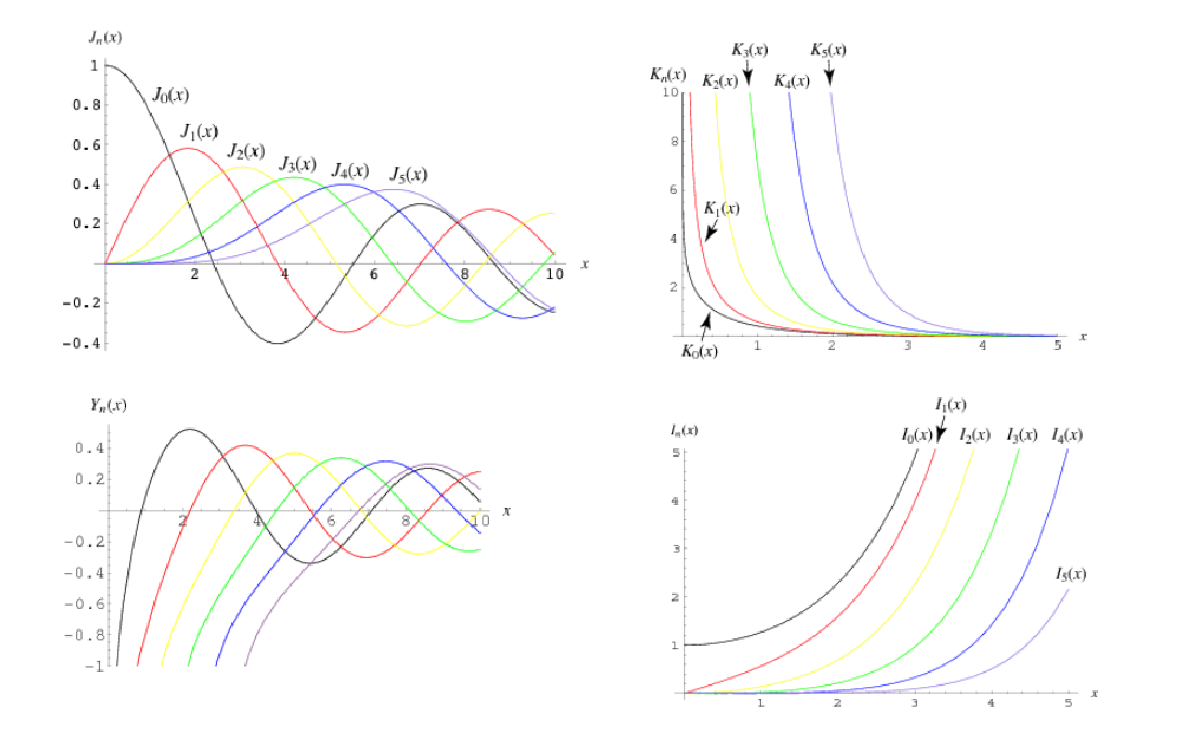
\includegraphics[width=120mm]{bessel.eps}
\tiny{\begin{verbatim}
                                       http://mathworld.wolfram.com
\end{verbatim}}
\end{frame}

%15
\begin{frame}
\frametitle{\textbf{Deriving a Solution:} Bessel's Equation}
\textbf{Equations obtained from curls $\vec{\nabla}\times\vec{E}$ and $\vec{\nabla}\times\vec{H}$ are combined:}
{\small \begin{align*}
E_\theta^{(core)}&=\frac{-i}{u^2}\left((Am\frac{\beta}{r}J_m(ur)+B\omega\mu_0\frac{\partial J_m(ur)}{\partial r}\right)\sin{(m\theta+\alpha)},\\
E_\theta^{(cladding)}&=\frac{-i}{w^2}\left(Cm\beta\frac{\partial K_m(wr)}{\partial r}+D\frac{\omega\mu_0}{r}\frac{\partial K_m(wr)}{\partial\theta}\right)\sin{(m\theta+\alpha)},\\
H_\theta^{(core)}&=\frac{-i}{u^2}\left(Am\frac{\beta}{r}J_m(wr)+B\omega\varepsilon_0 n_1^2\frac{\partial K_m(wr)}{\partial r}\right)\cos{(m\theta+\alpha)},\\
H_\theta^{(cladding)}&=\frac{-i}{w^2}\left(Cm\beta J_m(wr)+D\frac{\omega\varepsilon_0 n_0^2}{r}\frac{\partial K_m(wr)}{\partial\theta}\right)\cos{(m\theta+\alpha)}.
\end{align*}}
\textbf{Applying BCs for Maxwell's wave equations obtains:}
\hspace{-10mm}{\small \begin{equation*}
\left(\begin{array}{cccc}
\frac{m\beta}{u^2a^2}J_m(ua)&\frac{k\omega\mu_0}{ua}J'_m(ua)&\frac{m\beta}{w^2a}K_m(wa)&-\frac{k\omega\mu_0}{w^2a}K'_m(wa)\\
\frac{kn_1^2}{ua}J'_m(ua)&\frac{\omega\mu_0m}{u^2a^2}J_m(ua)&\frac{k^2n_0^2}{wa}K'_m(wa)&\frac{\omega\mu_0m\beta}{w^2a^2}K_m(wa)\\
J_m(ua)&0&-K_m(wa)&0\\
0&J_m(ua)&0&K_m(wa)
\end{array}\right)
\left(\begin{array}{c}A\\B\\C\\D\end{array}\right)=
\left(\begin{array}{c}0\\0\\0\\0\end{array}\right)
\end{equation*}}
\end{frame}

%16
\begin{frame}
\frametitle{\textbf{Deriving a Solution:} Characteristic Equation}
\begin{itemize}
\item \textbf{Characteristic equations} give solutions along light rays; given by determinant
\begin{equation*}
\left|\begin{array}{cccc}
\frac{m\beta}{u^2a^2}J_m(ua)&\frac{k\omega\mu_0}{ua}J'_m(ua)&\frac{m\beta}{w^2a}K_m(wa)&-\frac{k\omega\mu_0}{w^2a}K'_m(wa)\\
\frac{kn_1^2}{ua}J'_m(ua)&\frac{\omega\mu_0m}{u^2a^2}J_m(ua)&\frac{k^2n_0^2}{wa}K'_m(wa)&\frac{\omega\mu_0m\beta}{w^2a^2}K_m(wa)\\
J_m(ua)&0&-K_m(wa)&0\\
0&J_m(ua)&0&K_m(wa)
\end{array}\right|.
\end{equation*}
\item Families of solutions correspond to values of $m$ w.r.t. \textbf{one} of the fields $\vec{E}$ or $\vec{H}$.
\item Seek solution for modes satisfying $m=0$, called the TE and TM modes.
\end{itemize}
\end{frame}

\begin{frame}
\frametitle{\textbf{Conclusion:} TE and TM Modes}
\begin{itemize}
\item When $m=0$, the characteristic equation becomes
\begin{equation*}
\left(\frac{J'_0(ua)}{uaJ_0(ua)}+\frac{K'_0(wa)}{waK_0(wa)}\right)\left(\frac{J'_0(ua)}{ua J_0(ua)}+\frac{n_0^2}{n_1^2}\frac{K'_0(wa)}{wa K_0(wa)}\right)=0\nonumber.
\end{equation*}
\begin{equation*}
\mbox{with}\quad H_z=BJ_0(ur)\sin{(\alpha)},\qquad H_z=DK_0(wr)\sin{(\alpha)}
\end{equation*}
\item \textbf{Normalized frequency} is $$V=\sqrt{(wa)^2+(ua)^2}=\left[a\sqrt{n_1^2-n_0^2}\right]k=\left[a\sqrt{\mu_0\varepsilon_0(n_1^2-n_0^2)}\right]\omega$$
\item Since $n_1$ and $n_0$ are independent of frequency, the \textbf{normalized group velocity} is given by the product rule; $$\frac{d\beta}{d k}=\frac{a\sqrt{n_1^2-n_0^2}}{a\sqrt{n_1^2-n_0^2}}\frac{d(\frac{V\beta}{k})}{dV}=V\frac{d\left(\frac{\beta}{k}\right)}{dV}+\frac{\beta}{k}.$$
\end{itemize}
\end{frame}

\begin{frame}[fragile]
\frametitle{\textbf{Conclusion:} TE and TM modes}
\begin{columns}
\column{0.5\textwidth}
\includegraphics[width=\textwidth]{normFreqGroupVelocity.eps}
\column{0.5\textwidth}
\vspace{-10mm}{\tiny \begin{verbatim}
https://static.cambridge.org/resource/id/urn:cambridge
\end{verbatim}\vspace{-7mm}\begin{verbatim}
.org:id:binary:86398:20160620074821099-0818:02616fig3_
\end{verbatim}\vspace{-8mm}\begin{verbatim}
16.png?pub-status=liveg
\end{verbatim}}
\begin{itemize}
\item If $V>2.4$ then group velocity is non-zero for other modes with $m\neq 0$.
\item For sufficiently small $\omega$, only TE mode present.
\end{itemize}
\end{columns}
\begin{itemize}
\item Non-zero group velocity implies the corresponding mode propagates with a particular group velocity determined by its normalized frequency.
\item A dispersion mode with some value of $\omega$ in the solution propagates HE and EH modes with corresponding group velocities.
\end{itemize}
\end{frame}


\begin{frame}
\textbf{Can interpret dispersive properties with group velocity behaviour of modes w.r.t. source frequency.}
\frametitle{\textbf{Conclusion:} Hybrid Modes}
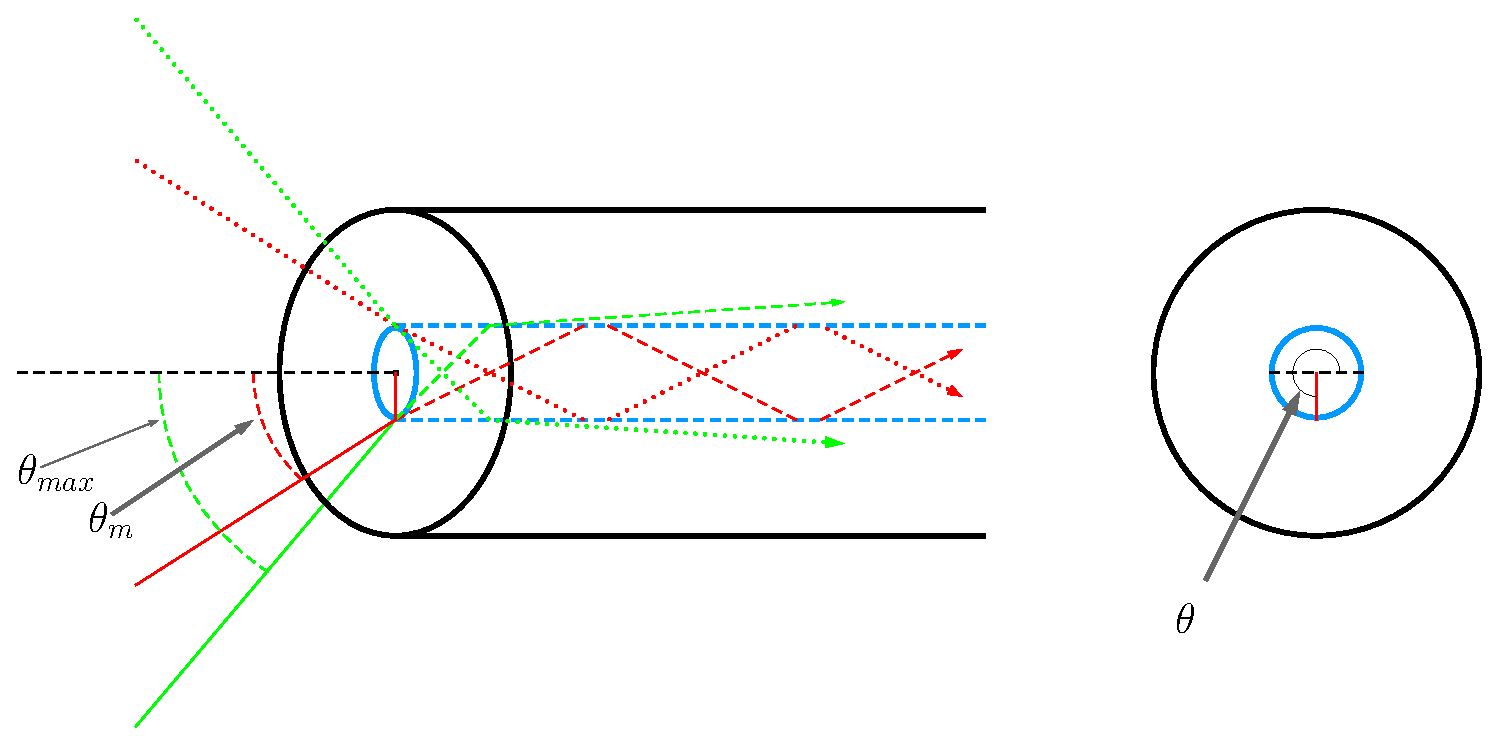
\includegraphics[width=12cm]{conclusionDiagram.eps}
\end{frame}

%\begin{frame}
%\frametitle{Blocks of Highlighted Text}
%\begin{block}{Block 1}
%\end{block}

%\begin{block}{Block 2}
%\end{block}

%\begin{block}{Block 3}
%\end{block}
%\end{frame}

%------------------------------------------------

%\begin{frame}
%\frametitle{Multiple Columns}
%\begin{columns}[c] % The "c" option specifies centered vertical alignment while the "t" option is used for top vertical alignment

%\column{.45\textwidth} % Left column and width
%\textbf{Heading}
%\begin{enumerate}
%\item Statement
%\item Explanation
%\item Example
%\end{enumerate}

%\column{.5\textwidth} % Right column and width
%X

%\end{columns}
%\end{frame}

%------------------------------------------------

%\begin{frame}
%\frametitle{References}
%\footnotesize{
%\begin{thebibliography}{99} % Beamer does not support BibTeX so references must be inserted manually as below
%\bibitem[Smith, 2012]{p1} John Smith (2012)
%\newblock Title of the publication
%\newblock \emph{Journal Name} 12(3), 45 -- 678.
%\end{thebibliography}
%}
%\end{frame}

%------------------------------------------------

\begin{frame}
\Huge{\centerline{The End}}
\end{frame}

%----------------------------------------------------------------------------------------

\end{document} 